This  design  requires   three   different  voltage  levels  (known  as  voltage
\emph{rails}),  which  are  \SI{28}{\volt},  \SI{5}{\volt}  and  \SI{3.3}{\volt}
respecitvely. Each rail has  different  requirements  as far as noise, power and
efficiency goes.

First  and  foremost,  the  maximum  current  of  each   voltage  rail  must  be
approximately determined. This information is crucial for  selecting appropriate
voltage regulators.

The most  power-hungry  component  on  the  \SI{3.3}{\volt}  rail is clearly the
dsPIC33   microcontroller   and  LEDs.   According   to   the   datasheet,   the
microcontroller will  consume  \SI{0.5}{\milli\ampere\per\mega\hertz}. Since the
microcontroller will be clocked  at  \SI{120}{\mega\hertz},  the minimum current
can be calculated with the following equation.
\begin{equation}
    I_{dsPIC} = \SI{0.5}{\milli\ampere\per\mega\hertz} \cdot \SI{120}{\mega\hertz} = \SI{60}{\milli\ampere}
\end{equation}
The other significant power-hungry components are the four LEDs connected to the
dsPIC33 microcontroller. Each consume \SI{15}{\milli\ampere}. The total  current
consumption of the \SI{3.3}{\volt} rail is therefore roughly:
\begin{equation}
    I_{\SI{3.3}{\volt}} = I_{dsPIC} + 4 \cdot \SI{15}{\milli\ampere} = \SI{120}{\milli\ampere}
\end{equation}

The \SI{3.3}{\volt} rail  derives  it's  voltage  from  the  \SI{5}{\volt} rail.
Additionally,  the OLED display is powered by  the  \SI{5}{\volt}  rail,  which,
according to the datasheet, draws a maximum  current of \SI{135}{\milli\ampere}.
The total  current  consumption of the \SI{5}{\volt} rail will approximately be:
\begin{equation}
    I_{\SI{5}{\volt}} = I_{\SI{3.3}{\volt}} + \SI{135}{\milli\ampere} = \SI{255}{\milli\ampere}
\end{equation}

A  decision  for  each  voltage rail must be made. Do we use a switch-mode power
regulator  or a linear regulator?  The  general  trade-off  is  that  swith-mode
regulators have  a  very  high  efficiency,  but  due  to the nature of how they
transform voltages, they produce a lot more jitter on the output. In contrast, a
linear regulator produces almost  no jitter -- in fact, it even dampens incoming
jitter  by  a substantial amount -- however, the linear regulator has very  poor
efficiency since  it  just  ``burns''  the  excess voltage and produces a lot of
heat,  making  it  a  poor  candidate  for transforming between  larger  voltage
differences.

The \SI{28}{\volt}  rail  is  already  taken care of, since that's precisely the
voltage the external power supply provides.

Seeing as  there  is  a very large voltage difference between \SI{28}{\volt} and
the next lower rail, \SI{5}{\volt}, a switch-mode regulator is clearly  the only
sane choice to be made for powering  the  \SI{5}{\volt}  rail  due to efficiency
reasons.   The    diagram   of   this   circuit   is   illustrated   in   figure
\ref{fig:circuit:rails}. There is little reason  to  discuss  the  selection  of
components of  this circuit in great detail; It's using a standard configuration
according  to  the  datasheet.  The  regulator  was  chosen based on the current
requirement $I_{\SI{5}{\volt}}$ and is capable of supplying a maximum current of
\SI{750}{\milli\ampere}.

All   digital   circuitry,  such  as   the   micro   controller,   operates   at
\SI{3.3}{\volt}. It is particularly important for the  \SI{3.3}{\volt}  rail  to
have as  little  noise/jitter  as possible. This requirement stems from the fact
that  the  analog-to-digital  (ADC)  conversions  and  digital-to-analog   (DAC)
conversions derive their  reference  voltage  from the \SI{3.3}{\volt} rail. Any
noise on  this  rail  could  impact  the accuracy of these conversions and could
result in lower accuracy of the final,  regulated  output  voltage of the device
itself.  For  this  reason  we  opted  for  a  linear  regulator  to  power  the
\SI{3.3}{\volt} off of the \SI{5}{\volt} rail.  the  circuit  is  illustrated in
figure  \ref{fig:circuit:rails}.  This regulator was also chosen  based  on  the
current requirement $I_{\SI{3.3}{\volt}}$ and is capable of  supplying a maximum
current of \SI{1}{\ampere}.

\begin{figure}[th!]
    \center
    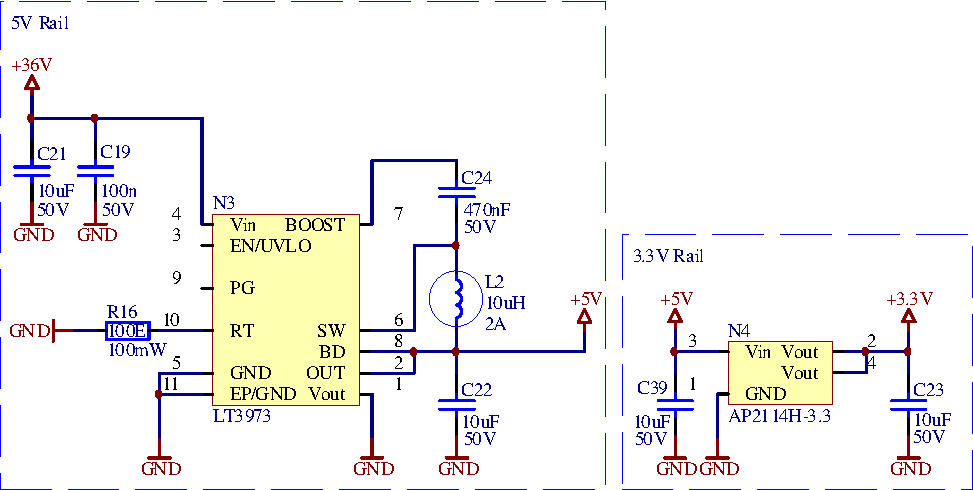
\includegraphics[width=.75\textwidth]{images/circuit/5v-3v-rails.pdf}
    \caption{Speisung f\"ur 5V mittels Abwertswandler (links) und Speisung f\"ur 3.3V mittels Linearregler (rechts)}
    \label{fig:circuit:rails}
\end{figure}

